\documentclass[11pt]{article} 

% ***********************************************************
% ******************* PHYSICS HEADER ************************
% ***********************************************************
% Version 2
%\usepackage{MnSymbol}
\newtheorem{guess}{Hypothesis}
%\usepackage[b5paper]{geometry}


\usepackage{mathtools}   % loads »amsmath«
\usepackage{empheq}


\usepackage{epsfig}
%\usepackage{mdframed}
\usepackage{tikz}
\usetikzlibrary{scopes}
\usepackage{amsmath}
\usepackage{bm}
\usepackage{amsthm } % Theorem Formatting
\usepackage{amssymb}	% Math symbols such as \mathbb
\usepackage{listings}

\usepackage{graphicx}

%\usepackage{hyperref}
\usepackage{multicol} % Allows for multiple columns

\usepackage{fullpage, float, subfig, verbatim,amsmath, mathrsfs}
\usepackage{fancyhdr}
\usepackage{natbib}
\usepackage{appendix}
\usepackage{alltt}
%%%%
\usepackage{breqn}
\usepackage{fixltx2e}

\sloppy
\definecolor{lightgray}{gray}{0.5}
%%%%
\fancyhf{}
\headsep=20pt

% algorithm
\usepackage{algorithm}
\usepackage{algorithmic}


\usepackage[glenn]{fncychap}
\usepackage{sectsty}
\allsectionsfont{\sffamily\mdseries\upshape} % (See the fntguide.pdf for font help)

%Change the chapte layout
\usepackage{titlesec}
\titlespacing*{\chapter}{0pt}{-50pt}{20pt}
\titleformat{\chapter}[display]{\ttfamily \LARGE\bfseries}{\chaptertitlename\ \thechapter}{20pt}{\Huge}

% Fancy MATLAB-kode:
\usepackage{textcomp}
\definecolor{lbcolor}{rgb}{0.95,0.95,0.95}
\lstset{
%	backgroundcolor=\color{lbcolor},
	tabsize=4,
	rulecolor=,
	language=matlab,
        basicstyle=\scriptsize,
        upquote=true,
        aboveskip={1.5\baselineskip},
        columns=fixed,
        showstringspaces=false,
        extendedchars=true,
        breaklines=true,
        prebreak = \raisebox{0ex}[0ex][0ex]{\ensuremath{\hookleftarrow}},
        frame=single,
        showtabs=true,
        showspaces=false,
        showstringspaces=false,
        identifierstyle=\ttfamily,
        keywordstyle=\color[rgb]{0,0,1},
        commentstyle=\color[rgb]{0.133,0.545,0.133},
        stringstyle=\color[rgb]{0.627,0.126,0.941},
        numbers=left, 
        numberstyle=\tiny, 
        stepnumber=1, 
        numbersep=5pt
}

% equations
\definecolor{myeqcolor}{gray}{0.9}
\newcommand*\mygraybox[1]{%
\colorbox{myeqcolor}{\hspace{1em}#1\hspace{1em}}}

% more equation highlightin
%\usepackage{framed}
\usepackage[framemethod=TikZ]{mdframed}
\usepackage{xcolor}
\surroundwithmdframed[
    hidealllines=true,
    backgroundcolor=black!20,
    skipbelow=\baselineskip,
    skipabove=\baselineskip
]{equation}
\global\mdfdefinestyle{graybox}{%
outerlinewidth=0pt,innerlinewidth=0pt,
outerlinecolor=gray,roundcorner=5pt,
backgroundcolor=gray!27
}

\usepackage{longtable}

%\usepackage[svgnames]{xcolor} % Required to specify font color

\newcommand*{\plogo}{\fbox{$\mathcal{PL}$}} % Generic publisher logo

%----------------------------------------------------------------------------------------
%	TITLE PAGE
%----------------------------------------------------------------------------------------

\newcommand*{\titleAT}{\begingroup % Create the command for including the title page in the document
\newlength{\drop} % Command for generating a specific amount of whitespace
\drop=0.1\textheight % Define the command as 10% of the total text height

\rule{\textwidth}{1pt}\par % Thick horizontal line
\vspace{2pt}\vspace{-\baselineskip} % Whitespace between lines
\rule{\textwidth}{0.4pt}\par % Thin horizontal line

\vspace{\drop} % Whitespace between the top lines and title
\centering % Center all text
%\textcolor{Red}{ % Red font color
{\Huge A TITLE}

\vspace{0.25\drop} % Whitespace between the title and short horizontal line
\rule{0.3\textwidth}{0.4pt}\par % Short horizontal line under the title
\vspace{\drop} % Whitespace between the thin horizontal line and the author name
by \\
\vspace{0.25\drop} % Whitespace between the thin horizontal line and the author name
{\Large \textsc{Simen Andresen}}\par % Author name
\vfill % Whitespace between the author name and publisher text

NTNU
\rule{\textwidth}{0.4pt}\par % Thin horizontal line
\vspace{2pt}\vspace{-\baselineskip} % Whitespace between lines
\rule{\textwidth}{1pt}\par % Thick horizontal line

\endgroup}



\linespread{1.5}




% algorithms
\floatstyle{plain}
\newfloat{myalgo}{tbhp}{mya}

\newenvironment{Algorithm}[2][tbh]%
{\begin{myalgo}[#1]
\centering
\begin{minipage}{#2}
\begin{algorithm}[H]}%
{\end{algorithm}
\end{minipage}
\end{myalgo}}

% then use the following
		%\begin{Algorithm}[t]
		%\caption{Does work, though no nice solution.}
		%\end{Algorithm}

%\newcommand{\textpath}{./texts/}



%%%%%%% TITLE %%%%%%%%%%%%%%%%%%%%%

\title{My title}
\author{Simen Andresen}
\date{\ \\ \ \\ \today}

%%%%%%%%%%% DOCUMENT %%%%%%%%%%%%%
\begin{document}

\captionsetup{width=0.8\textwidth}

% custom commands - variables etc
\newcommand{\bs}{\boldsymbol}
\newcommand{\taub}{\bs \tau}
\newcommand{\vdotbb}{\dot{\bs V}_{0b}^B}
\newcommand{\vdotb}[2]{\dot{\bs V}_{#1}^#2}
\newcommand{\vbb}{\bs V_{0b}^B}
\newcommand{\vb}[2]{\ensuremath{\bs V_{#1}^#2}}
\newcommand{\jg}[2]{\ensuremath{\bs J_{#1}^#2}}
\newcommand{\qdot}{\dot{\bs q}}
\newcommand{\xidotb}{\dot{\bs \xi}}
\newcommand{\xib}{\bs \xi}
\newcommand{\zetab}{\bs \zeta}
\newcommand{\zetadotb}{\dot{\bs \zeta}}
\newcommand{\etab}{\ensuremath{\bs \eta}}
\newcommand{\etadotb}{\ensuremath{\dot{\bs \eta}}}
\newcommand{\adg}[1]{\ensuremath{\bs{Ad}_{g_{#1}}}}
\newcommand{\adgb}{\ensuremath{\bs{Ad}_{g_{0b}}}}
\renewcommand{\frame}[1]{\ensuremath{\mathcal{F}_{#1}}}
\newcommand{\Real}[1]{\ensuremath{\mathbb{R}^{#1}}}
\newcommand{\rb}[1]{\ensuremath{\bs R_{#1}}}
\newcommand{\pb}[1]{\ensuremath{\bs p_{#1}}}
\newcommand{\jb}[2]{\ensuremath{\bs J_{#1}^{#2}}}

\pagestyle{empty}
\titleAT

\
\cleardoublepage



 %%%%%%%%%%%%% BODY %%%%%%%%%%%%%%
\pagestyle{plain}

\pagenumbering{roman} % Roman numerals
\setcounter{page}{1}
\subsection*{Acknowledgement}

\clearpage


\subsection*{Preface}

\clearpage


\abstract


\clearpage


\section*{Notation and Acronyms}

\subsection*{Acronyms}
%acronyms
    \begin{longtable}{p{6cm}p{10cm}}
		AUV & Autonomous underwater vehicle
		\\
		DH & Denavit-Hartenberg 
		\\
		ROV & Remotely operated vehicle 
		\\
		UVMS & Underwater Vehicle-Manipulator System


    \end{longtable}
\subsection*{Mathematical symbols}
%math
%\begin{table}[h!]
    \begin{longtable}{p{6cm}p{10cm}}
			n & Number of links of the manipulator \\
			m & Number of degrees of freedom of the vehicle.  \\
			$\bs J \in \Real{6\times (m+n)}$ & $\bs J$ without superscripts or subscripts is always the jacobian mapping the quasi-velocities $\zeta$ to the body velocity of the end effector\\
			$\bs \omega_{0b} \in \Real 3$ & Rotational velocity of vehicle as observed from body frame.  \\
			$\bs J^{\dagger} \in \Real{(m+n) \times 6}$ & Pseudo-inverse of $\bs J$\\
			$\bs V_{0b}^{B} \in \Real 6  $ & Body velocity twist of vehicle\\
			$\bs V_{0b}^{S}\in \Real 6 $ & Spatial velocity twist of vehicle\\
			$\bs V_{0e}^{B}\in \Real 6 $ & Body velocity twist of end effector\\
			$\bs V_{0e}^{S}\in \Real 6 $ & Spatial velocity twist of end effector\\
			$\tau_{c} \in \Real{m+n}$ & Controlled input generalized forces\\
			$\bs \eta = \begin{bmatrix} (\bs \eta_{1})^{T} & (\bs \eta_{2})^{T}\end{bmatrix}^{T} \in \Real 6$  & Position and rotation (euler angles) of the vehicle, relative to an inertial frame \\
			$\bs \eta_{e} \in \Real 6$ & Position and rotation of end effector relative to inertial frame \\ 
			$\bs \xi = \begin{bmatrix} (\bs \eta)^{T} & (\bs q)^{T}\end{bmatrix}^{T} \in \Real {m+n} $ &  Configuration of UVMS \\
			$\bs \zeta = \begin{bmatrix} (\vb{0b}{B})^{T} & (\dot{\bs q})^{T}\end{bmatrix}^{T} \in \Real{m+n}$ & Velocities of the vehicle and manipulator arm. \\
			$\bs J_{a} \in \Real{(m+n) \times (m+n)} $ & Analytical Jacobian. Mapping quasi-velocities to the time derrivative of the general coordinates. \\
			$ \adg{0i}$ & Adjoint map matrix operator. \\
			$\jg{gi}{B} \in \Real{6 \times (m+n)}$ & Geometric Jacobian. Mapping quasi velocities to velocities of frame \frame i\\
			$\jg{ge}{B} \in \Real{6 \times (m+n)}$ & Geometric Jacobian. Mapping quasi velocities to velocities of end effector\\
			$\bs F_{e}^{e} \in \Real 6 $ & Force on end effector from interaction with the environment \\
			$|| \cdot ||$ & The 2 norm operator	 \\
			$|| \cdot ||_{\infty} $ & The infinity norm operator	



			
			

    \end{longtable}
%\end{table}




\clearpage


\cleardoublepage
\tableofcontents
\cleardoublepage

\pagenumbering{arabic} % Roman numerals
\pagestyle{fancy}
\chead{Underwater Robotics}
\rhead{\sectionmark}
\setcounter{page}{1}

\lfoot{\thepage}





\section{Introduction}

\clearpage
\section{Litterature Review}

In this section, different litterature on the topic of underwater vehicles with manipulators (UVMS) is presented. To focus is mostly on kinematics and force control solutions, but also some general modeling and motion control is presented.  
\\

\subsection{Antonelli G. - Underwater robotics}

\cite{antonelli1} presents mathematical models of the UVMS kinematics and dynamics, as well as motion control strategies for both the vehicle, and the total system, including a manipulator arm. For motion control, several strategies using adaptive control, is presented, where the controller adapts on a minimal set of parameters. Simulations is used to show the effectiveness of both the motion control, as well as for the kinematic control. Mathematical models for well known research UVMS's are used, facilitating the process of compareing control strategies. 
% kinematics

A real-time kinematic control is proposed for the total veichle-manipulator system, exploiting the redundancy in the system. This is generalized for an ROV with the normal 6 DOFs and with a m-link manipulator giving the system a total of $6+m$ DOFs. 
\cite{antonelli1} proposes a Closed-Loop Inverse Kinematic Algorithm for solving the inverse kinematics\footnote{Inverse kinematics will be explained later in this paper. In short it is the process of mapping end effector velocities to vehicle and joint velocities}. The algorithm uses feedback from the resulting position of the end effector to correct for the numerical drift in the method. The inverse velocity kinematics is solved with the following

\begin{align}
\label{eq:antIK}
\bs \zeta_r &=\bs J_{p}^{\dagger}(\bs \eta,\bs q) \left( \dot{\bs x}_{p,d} + \bs K_{e} \bs e_{e} \right) + \left( \bs I_N - \bs J_{p}^\dagger(\bs \eta,\bs q) \bs J_{p}(\bs \eta,\bs q)  \right)\bs J_{s}^\dagger(\bs \eta,\bs q) \left(\dot{\bs x}_{s,d} + \bs K_{s}e_{s} \right)
\end{align}
Where $ \dot{\bs x}_{p,d}$ and  $ \dot{\bs x}_{s,d}$ are the primary and secondary task coordinates, representing the end effector and vehicle velocities respectively. The matrices $\bs J_p$ and $ \bs J_s $ is the mapping from the vehicle and joint positions to the primary and secondary task coordinates. $\bs J^{\dagger}$ is the Moore-Penrose pseudo inverse of $\bs J$. The vectors $\bs K_{e}\bs e_{e}$ and $ \bs K_{s}\bs e_{s}$ are the weighted  position error of the primary and secondary tasks respectively.
The primary task is defined as the planned velocity of the end effector, while the secondary task is the desired motion of some internal element of the kinematics chain, e.g. the vehicle, that does not change the end effector velocity.

\cite{antonelli1} also presents a fuzzy inverse kinematics law, based on the weighted pseudo inverse

\begin{align}
	\bs J_{w}^{\dagger} &= \bs W^{-1} \bs J^{T} \left( \bs J \bs W^{-1}\bs J^{T} \right)^{-1}
	\label{eq:wpseudo}
\end{align}

The weighted pseudo inverse is widely used in robotics, as a robust way of avoiding joint limits by weighting the diagonal elements of $\bs W$ according to how close they are to a limit. In \cite{antonelli1}, the weighing matrix $\bs W$ is used to distribute the motion between the manipulator and the vehicle. This is done in order to avoid unescessary motion of the vehicle, yielding a more energy effective approach, due to the vehicles large inertia, relatice to the manipulator.

% end antonelli

% kim two time scale
\subsection{Kim et al. -  Dynamic Analysis and Two-Time Scale Control for
Underwater Vehicle-Manipulator Systems}

\cite{two_time_scale} proposes a control scheme that takes the different bandwidth of the manipulator and vehichle into account for a generalized UVMS with a $n$-link manipulator. This is favourable since the bandwidth of the vehichle is naturally much lower due to it's larger inertia. The proposed control scheme is an active damping control with two-time scale approach in operational space. The basic consept is to control the vehichle alone using a passive or simply a proportional (P) control, and a two-time scale controller for the manipulator to control the total UVMS. 

The vehichle is represented in a partially linear form, and the vehichle is controlled using
\begin{align}
  \bs \tau_v &= - \bs J_{v}^{-1}(\bs \eta)\bs K_v \bs \eta
  \label{eq:kimProp}
\end{align}
Where $\bs J_v(\bs \eta)$ is defined as $\etadotb=\bs J_v(\etab)\vbb $. By including the controller in the partially linearized dynamics of the UVM system the manipulator control law is proposed as a feedback linearizing controller:
\begin{align}
  \bs \tau_m &=\bs M^* \bs u+ \bs h^*
  \label{eq:kim_feedback_lin}
\end{align}
By including \eqref{eq:kim_feedback_lin} the system yields:

\begin{align}
  \bs M_{11}  \vdotbb + \bs J_v^{-1} \bs K_v \bs \eta &= -\bs M_{12} \bs u
  \label{eq:kim_linearized} \\
  \bs{\ddot q} &=\bs u
  \label{eq_kim_linearized2}
\end{align}
For a definition of the inertia matrices $M_{11}$ and $M_{12}$ the reader are refered to \cite{two_time_scale}. Further the control input $u$ is defined as $\bs u = \bs u_{slow}+\bs u_{fast}$ where the slow part mainly affects the vehichle dynamics, while the fast part mainly affects the manipulator. $\bs u_{fast}$ is then designed as a high gain linear tracking controller yielding a frequency much higher than the bandwidth of the vehichle. The controller scheme is tested on ODIN \footnote{ODIN(Omni-Directional Intelligent Navigator) is a underwater robot developed at the Autonomous Systems Laboratory of the University of Hawaii} with a 3 DOFs manipulator, showing good tracking results.  


\subsection{Fossen et al. - Modeling and Control of Underwater Vehicle-Manipulator Systems }

\cite{foss_schjolberg_modelling} presents a mathematical model of a UVMS system, with an in depth description of most of the hydrodynamic terms. The mathematical model is separates between the manipulator dynamics and the vehicle dynamics by adding the forces of interaction between them.

proposes a control law for the UVM system utilizing feedback linearization. The number of DOFs of the manipulator is not specified, but the refered manipulator jacobian is invertible and it is therefor reasonable to assume a 6 DOFs manipulator. The idea of the controller is to feedback the nonlinear terms acting on the ROV and the manipulator independently, and further use a PID feedback yielding exponential tracking error dynamics in both the manipulator and the vehichle. The proposed controller yields the closed loop control for the vehicle

\begin{align}
	\bs \tau_{r} & = \bs M_{11}(\bs q) \bs a_{v} + \bs M_{c}(\bs q) \ddot{\bs q} + \bs n_{1} \\
	\bs a_{v} &= \ddot{\bs \eta}_{d} - \bs K_{p} \tilde{\bs \eta} - \bs K_{d} \dot{\tilde{\bs \eta}} + \bs n_{1} \left( \bs q, \dot{\bs q},\bs \nu \right)
	\label{eq:fossenfbl}
\end{align}
$\bs n_{1}$ is then the vector containing all the nonlinearities of the vehicle. The control input to the manipulator $\bs \tau_{m}$ is defined in the same way. 



\subsection{Han et al. - 
Redundancy Resolution for Underwater Vehicle-Manipulator Systems
with Minimizing Restoring Moments }

\cite{redundancy_res_restoring_forces} Proposes a redundancy resolution of UVM systems which minimizes the restoring moments. The freedom of motion in the nullspace of the end effector can then be used to position the vehichle in a way that is advantagous to the energy consumption of the UVMS. This is especially favourable when the system is run by battery, and hence minimizing energy consumption is essential.
The proposed inverse kinematic uses the weighted pseudo inverse and projects the vector $z$ into the nullspace of the jacobian $\bs J$ 
\begin{align}
  \xidotb&=\bs J^{W \dagger} \dot{\bs x}_E^0+(\bs I- \bs J^{W \dagger})\bs z
  \label{eq:restoringforces_inverse}  \\
  \bs J^{W \dagger}&= \bs W^{-1} \bs J^T  \left( \bs J \bs W^{-1} \bs J^T \right) ^{-1}
  \label{eq:restoring_J}
\end{align}
Where an arbitrary velocity vector $\bs z\in \mathbb{R}^{6+n}$ is projected in the null space of the end effector Jacobian and $\bs W$ is any positive definite weight matrix, in the same way as proposed in \cite{antonelli1}. 
The vector $z$ is then the gradient projection direction of a cost function $\phi$ which measures the systems performance to minimize the restoring moments of the vehicle. The proposed cost function is

\begin{align}
	\phi &= \frac{1}{2} || \bs r_{g} - \bs r_{b} ||
	\label{eq:minimizingrestoring}
\end{align}
Where the vectors $\bs r_{g}$ and $\bs r_{b}$ are the vectors representing the center of gravity and boyancy, respectively. The paper presents simulation results, yielding good results in saving energy.







\subsection{Yong Cui \& Niljanjan Sarkar - A Unified Force Control Approach to Autonomous}
Underwater Manipulation
\cite{unified_force_control} proposes a unified force control law for an UVM system. The UVM system is generalized for a 6 DOFs underwater vehicle and an 3-link arm. The paper includes a model of the total system, without taking the current effect into account. The controller is based on hybrid force/position and impedance control, and is supposed to keep a stable contact with the environment as well as tracking desired force trajectories without the knowledge of the environment. The paper distinguishes the three phases of operation: 


\begin{itemize}
  \item No contact with environment
  \item Transition phase
  \item Contact with environment
\end{itemize}
Because of the difference of control in the three phases, a fuzzy rule is proposed to identify and switch control between the different phases. The system is modeled in the task space of the end effector motion with pose $\bs X$
\begin{align}
  \tilde{\bs M}\ddot{\bs X}  + \tilde{\bs \zeta} = \bs F - \bs F_e
	\label{eq:unified_model} 
\end{align}
Where $\tilde{\bs \zeta}$ collects the coriolis, hydronanymic and gravitational forces, $\bs F$ and $\bs F_e$ is the controlled force and the force from the environment, respectively. The proposed control $\bs F_c $ is

\begin{align}
  \bs F_c &=\bs F_{IP}W + \bs F_H(1-W )+ \hat{\tilde{\bs \zeta}} + \bs F_e 
  \label{eq:unified_force}
\end{align}
Where $\bs F_{IP}$ is the output of an impedance controller,$\bs F_{H}$ is the output of a hybrid force/position controller, $\hat{\tilde{\bs \zeta}}$ is an estimate of $\tilde{\bs \zeta}$ and $W$ is the weight variable, controlled by the fuzzy logic.

The purpose of the fuzzy law tuning the weight $W$ is to keep a smooth transition between the three states. Especially in the transition phase it is difficult to keep a good model of the UVMS. When the UVMS operates in the no contact phase, it is only controlled with an impedance control which is obtained by $W=1$. The impedance controller is based on the work done in \cite{impedance_stability}, and has the following structure

\begin{align}
  \bs  F_{IP} &= \hat{\tilde{\bs M}}\bs U % \hat{\tilde{\bs \zeta}} + \bs F_e
  \label{eq:impedance_control}
\end{align}
Where the hat operator indicates the estimate of the variables, and $\bs U$ is the commanded acceleration giving the desired impedance:

\begin{align}
  \bs U&=\ddot{\bs X}_d + \bs P^{-1}\left[ \bs B_d(\dot{\bs X}_d-\dot{\bs X}) + \bs K(\bs X_d - \bs X) - \bs F_e\right]
  \label{eq:impedance_control2}
\end{align}
Where $\bs P$, $\bs B_d$ and $\bs K$ gives the desired impedance relationship between the end effector and the environment. Further the hybrid position/force command $\bs F_H$ in \eqref{eq:unified_force} is based on the following

\begin{align}
  \bs F_H&= (\bs I - \bs S)\bs F_p + \bs S \bs F_f
  \label{eq:hybrid1}
\end{align}
Where $\bs S$ is the compliance selection matrix selecting which directions in the task space force control should be applied and which directions position control should be applied. $\bs F_p$ and $\bs F_f$ is the output from PID and PI controllers, controlling the position and force respectively.


The fuzzy rule tunes W according to the state of the system in terms of the ratio of $\frac{\bs F_e}{\bs F_d}$  and $\bs \nu_e$ where $\bs \nu_e$ and $\bs F_d$ is the desired velocity and force at the end effector. 
Numerical simulations are done yielding good results of motion between no contact and contact operations. 





\subsection{Agility for Underwater Floating Manipulation: Task \& Subsystem Priority Based Control Strategy}
The paper from \cite{trident_1} presents interesting results from the control methodology used in the EU-FP7 TRIDENT project. Trident is based on cooperation between an Unmanned Surface Craft(USC), and an AUV with manipulator capabilities, yielding many interesting possibilities especially with respect to navigation. The Trident is aimed to develop a multipurpose Intervention AUV (I-AUV) for used for intervention in unstructured underwater environments (\cite{trident1}).The I-AUV consists of a controlled AUV which constitutes the floating base of a redundant manipulator manipulator.  The main objectives in \cite{trident_1} is to avoid joint limits in the manipulator, to keep the end effector in a dexterous pose visible for the camera, and finally to get the end effector in the position to e.g. grasp an object. This is done by  

\newcommand*{\mybox}[2]{\colorbox{#1!30}{\parbox{.98\linewidth}{#2}}}





\section{Modelling}

In this section mathematical models of the UVMS is presented. The kinematics of the UVMS is highly complex due to the mix of quasi-velocities and generalized velocities, and the number of degrees of freedom of the total system. 
The dynamics is also highly complex, due to the high amount of parameters in the hydrodynamics, strong coupling forces between the rigid bodies, varying inertia for different manipulator configuration and more. The kinematics can be derived in the framework of Lie groups and Lie algebras. However, a detailed study of this is not included, but can be found in e.g. \cite{kristin_jant}. It should be noted that some of the notation is not consistent with the  litterature of underwater vehicles, due to the need to be consistent within the framework of the UVMS when refering to velocities. Instead of refering to the body velocity of the ship as $ \bs \nu$, the notation $ \vb{0b}{B}$ is used in order to comply with the notation used for velocities of the other frames in the UVMS. 
 

%kinematics
\subsection{Kinematics}

\begin{figure}[h!]
  \centering
  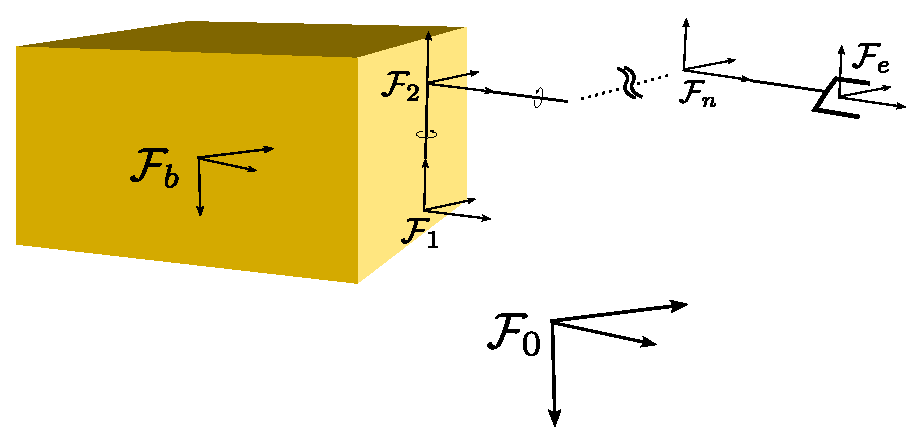
\includegraphics[scale=0.6]{./figures/uvms_kinematics.eps}
  \caption{The assignment of the frames for the UVMS system}
  \label{fig:uvms_kinematics}
\end{figure}
The ROV is regarded as a rigid body with the normal 6 degrees of freedom (DOFs), and the manipulator is a 6-link kinematic chain with only 1 DOF revolute joints. For representing the kinematic structure of the UVM system, a number of frames are assigned as shown in Fig. \ref{fig:uvms_kinematics}. A reference frame $\mathcal{F}_0$ is attached to the earth and is considered inertial. The body frame is located at the ROV's center of mass while the frames of the manipulator is attached according to the Denavit-Hartenburg (DH) convention \cite{spong2005robot}. 

\begin{figure}[h!]
	\centering
	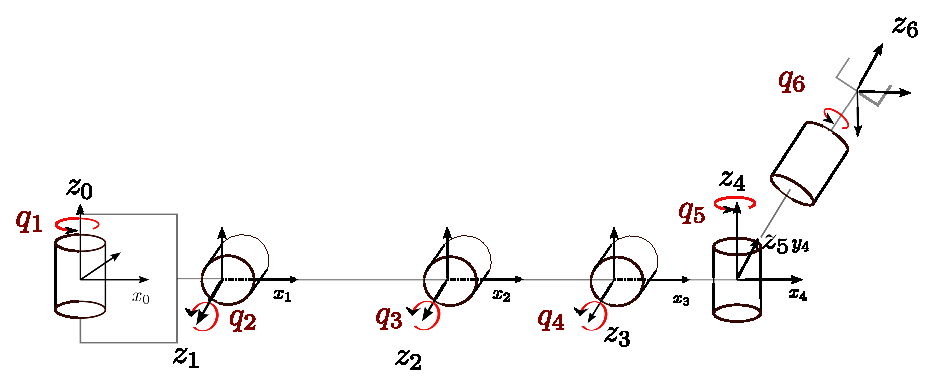
\includegraphics[scale=0.7]{./figures/manipulator_kinematics.eps}
	\caption{The frames are assigned to the kinematic structure of the manipulator according to the DH convention}
	\label{fig:dh-manipulator}
\end{figure}
For representing the orientation of the vehichle euler angles are used, which gives a minimal representation of the attitude at the expense of giving representational singulatities, see e.g. \cite{fs}. The position is represented as the coordinates of the origin of $\mathcal{F}_b$ relative to $\mathcal{F}_0$. The configuration of the manipulator are represented using the angles $q$. The total configuration given in generalized coordinates can then be written in vector form.
\begin{align*}
  \xib&:= \left[ \etab^T \bs q^T \right]^T \in \mathbb{R}^{6+n}
  \\
  \etab &= \begin{bmatrix}\etab_1 \\ \etab_2 \end{bmatrix}  = \begin{bmatrix} x_{0b} \\ y_{0b} \\ z_{0b} \\ \phi \\ \theta \\ \psi \end{bmatrix} \in \mathbb{R}^{6}
\end{align*}
One of the challenges to UVM systems is the mix of euclidean and non euclidean transformations representing the configuration of the system. While the transformation of each link is euclidean, the transformation of the vehicle is non-Euclidean \footnote{see i.e. \cite{kristin_jant} for a detailed discussion} , and in general the following is true
\begin{align}
	\bs \omega_{0b} \neq & \etadotb_2
  \label{eq:quasi1}
\end{align}
We will therefor use quasi-velosities $ \zetab $ or $\zetab^S$ to represent the velocity state of the system
\begin{align}
  \zetab &= \begin{bmatrix} \vbb \\ \qdot \end{bmatrix}
  \label{eq:zeta1}
	\\
	\zetab^S &= \begin{bmatrix} \vb{0b}{S} \\ \qdot \end{bmatrix}
	\label{eq:zetas}
\end{align}
Where $\vbb = \begin{bmatrix} \bs v^{T} & ( \bs \omega_{0b}  )^{T} \end{bmatrix}=  \begin{bmatrix} u & v & w & p & q & r \end{bmatrix}^T \in \mathbb{R}^6 $ is the body velocity twist, and $\zetab^S$ is the corresponding Spatial velocities as defined in \cite{kristin_jant}. The quasi coordinates can be mapped to the time derivative of the generalized coordinates through, \cite{kristin_jant} 
\begin{align}
 	\xidotb &=\bs J_a(\etab_2)\zetab 
  \label{eq:quasi_trans}
  \\
  \bs J_a &= \begin{bmatrix} \bs R_{0b}(\eta_2) & 0& 0 \\ 0 & \bs T_{0b}(\eta_2) & 0 \\ 0 & 0 & I \end{bmatrix} \in \mathbb{R}^{(6+n) \times (6+n) }
  \label{eq:jacobian_a}
\end{align}
Where $\bs T_{0b}(\eta_2)$ is written as in \cite{fs}.
\begin{align}
	\dot{\bs \eta}_2 & = \bs T\left( \bs \eta_{2} \right) \bs \omega_{0b}^{b} \\
	\bs T\left( \bs \eta_{2} \right) &= 
		\begin{bmatrix} 1 & s\phi t\theta & c\phi t\theta \\
										0 & c\phi & -s\phi \\
										0 & \frac{s\phi}{c\theta} & \frac{c\phi}{c\theta}
	\end{bmatrix}
	\label{eeq:fossen-transfomrm}
\end{align}
Where $s \; \cdot = sin(\cdot ), \; c \; \cdot = cos(\cdot)$ and $t \; \cdot = tan(\cdot)$. Throughout the paper several velocity variables will be used, so it is appropriate with a definition


\begin{mdframed}[style=graybox]
\begin{align}
&	\vb{0e}{B}\; - \; \text{Velocity of the end effector frame \frame e relative to \frame 0 as seen from \frame e} \nonumber
\\
& \vb{0b}{B}\; - \; \text{Velocity of \frame b relative to \frame 0 as seen from the vehicle frame \frame b} \nonumber
\\
&	\vb{0e}{S}\; - \; \text{Velocity of \frame e relative to \frame 0 in spatial coordinates relative to \frame 0} \nonumber
\\
&	\vb{0b}{S}\; - \; \text{Velocity of \frame b relative to \frame 0 in spatial coordinates relative to \frame 0} \nonumber
\end{align}

\end{mdframed}



Using the notation from \cite{kristin_jant} we define the body joint twist of a revolute joint as 
\begin{align}
	\bs X_i^i&=\begin{bmatrix} 0&0&0&0&0&1\end{bmatrix}^T
	\label{eq:body_twist}
\end{align}
It should be noted that the twist only has one nonzero component in the angular motion around the z axis due to following the Denavit-Hartenberg (DH) convention. It should also be noted that the body joint twist represents the direction of allowed motion seen from the body of link i, and is therefor always constant.
Next we define the spatial joint twist of a revolute joint as the allowed motion of each link relative to the frame $\mathcal{F}_0$, as written in \cite{kristin_jant}
\begin{align}
	\bs X_i&=\adg{0i}\bs X_i^i
	\label{eq:spatioal_twist}
\end{align}
Where the adjoint map between two frames \frame a and \frame b is defined as
\begin{align}
	\adg{ab}  &= \begin{bmatrix} \bs R_{ab} & \widehat{\bs p}_{ab}\bs R_{ab} \\ \bs 0 & \bs R_{ab} \end{bmatrix}
	\label{eq:adjoint}
  \\
	\adg{ab}^{-1} &= \begin{bmatrix} \rb{ab}^T & - \rb{ab}^T \widehat{\bs p}_{ab} \\ 0 & \rb{ab}^T \end{bmatrix}
	\label{eq:adjoint2}
\end{align}
Where \rb{ab} is the rotation matrix from \frame{a} to \frame{b}, and \pb{ab} is the vector representing the linear displacement of the origo of \frame b wrt. to \frame a. It should be noted that \adg{ab} can be seen as a map from body velocity \vb{ab}{B} to spatial velocity \vb{ab}{S}.
The hat operator $\widehat{(\cdot)}$ maps a vector to it's skew symmetric matrix representation, and when operating on a vector $\bs \omega \in \mathcal{R}^3$ is defined as
 \begin{align}
   \widehat{\bs \omega}&= \begin{bmatrix} 0 & -\omega_3 & \omega_2 \\ \omega_3 & 0 & -\omega_1 \\ -\omega_2 & \omega_1 & 0 \end{bmatrix} 
   \label{eq:skewsym}
 \end{align}
Using  \eqref{eq:adjoint} and \eqref{eq:body_twist} we get

\begin{align}
	\bs X_i&=\begin{bmatrix}\rb{0i} & \widehat{\bs p}_{0i} \rb{0i} \\ \bs 0 & \rb{0i}^T \end{bmatrix}\bs X_i^i
	\label{eq:adjoint_calc}
	\\
	&= \left[\begin{smallmatrix}{}r_{11} & r_{12} & r_{13} & p_{2} r_{31} - p_{3} r_{21} & p_{2} r_{32} - p_{3} r_{22} & p_{2} r_{33} - p_{3} r_{23}\\r_{21} & r_{22} & r_{23} & - p_{1} r_{31} + p_{3} r_{11} & - p_{1} r_{32} + p_{3} r_{12} & - p_{1} r_{33} + p_{3} r_{13}\\r_{31} & r_{32} & r_{33} & p_{1} r_{21} + p_{2} r_{11} & p_{1} r_{22} + p_{2} r_{12} & p_{1} r_{23} + p_{2} r_{13}\\0 & 0 & 0 & r_{11} & r_{12} & r_{13}\\0 & 0 & 0 & r_{21} & r_{22} & r_{23}\\0 & 0 & 0 & r_{31} & r_{32} & r_{33}\end{smallmatrix}\right]
	\left[  \begin{smallmatrix}0\\0\\0\\0\\0\\1 \end{smallmatrix}  \right]
	\\
	&=\left[\begin{smallmatrix}{}p_{2} r_{33} - p_{3} r_{23}\\- p_{1} r_{33} + p_{3} r_{13}\\p_{1} r_{23} + p_{2} r_{13}\\r_{13}\\r_{23}\\r_{33}\end{smallmatrix}\right]
\end{align}
Next we want to find a map from the generalized and quasi velocities to the velocities of each frame $\mathcal{F}_i$ with respect to the inertial frame \frame 0 in spatial coordinates. We also note the mapping between spatial and body velocities
\begin{align}
	\bs V_{0i}^S &=  \adg{0i} \bs V_{0i}^B  
  \label{eq:adg0b1}
 \end{align}
Following the notation in \cite{kristin_jant} we write the mapping from the velocities $\zetab$ to the velocities of frame $\mathcal{F}_i$ in both spatial and body coordinates
\begin{align}
	\vb{0i}{S}&= \jb{gi}{S}(\xib)\zetab^S
  \label{eq:spatial_jacobi}
  \\
	\jb{gi}{S}(\xib) &= \begin{bmatrix} \adg{0b} & \adg{0b} \bs J_i\end{bmatrix}
  \label{eq:spatial_jacobi2}
	\\
	\vb{0i}{B}&= \jb{gi}{B}(\xib)\zetab
  \label{eq:body_jacobi}
  \\
	\jb{gi}{B}(\xib) &= \begin{bmatrix} \adg{bi}^{-1} & \adg{bi}^{-1} \bs J_i\end{bmatrix}
  \label{eq:body_jacobi2}
\end{align}
Where $\bs J_i$ is the spatial geometric Jacobian of link i as written in \cite{kristin_jant} mapping the joint velocities to the spatial twist of link $i$
\begin{align}
  \bs V_{bi}^S &=\bs J_i(q)\dot q
  \label{eq:mappint1}
	\\
	\bs J_i&=\begin{bmatrix}  \bs X_1 & \bs X_2 & \cdots & \bs X_i & \bs 0_{6 \times (n-i)}    \end{bmatrix}
	\label{eq:Ji}
\end{align}
From \eqref{eq:spatial_jacobi} and \eqref{eq:body_jacobi} we get that the end effector velocity can be described using the following
\begin{align}
	\vb{0e}{S} &= \jb{ge}{S}\zetab^S
	\label{eq:ee_velo}
	\\
	&=\begin{bmatrix} \adg{0b} & \adg{0b}\jb{n}{}\end{bmatrix}\zetab^S
	\\
	\vb{0e}{B} &= \jb{ge}{B}\zetab
	\label{eq:ee_velo_body}
	\\
	&= \begin{bmatrix} \adg{bi}^{-1} & \adg{bi}^{-1} \bs J_n\end{bmatrix}\zetab
\end{align}
Where \jb{n}{} is defined in \eqref{eq:Ji} with $i=n$. We can now summarize the velocity kinematics
\begin{mdframed}[style=graybox]
	\begin{align}
	\vb{0i}{S}&=\jb{gi}{S}\zeta^S \\
	\vb{0e}{S}&=\jb{ge}{S}\zeta^S \\
	\zetab^S&=\begin{bmatrix} (\vb{0b}{S})^T & (\qdot)^T \end{bmatrix}^T \\
	\zetab^B&=\begin{bmatrix} (\vb{0b}{B})^T & (\qdot)^T \end{bmatrix}^T \\
	\vb{0i}{S}&=\adg{0i}\vb{0i}{B}
\end{align}
\end{mdframed}
%dynamics

\subsection{Dynamics}
The dynamics of the UVMS describes the motion of the vehicle in terms of forces, pose, velocities, and acceleration. The mathematical models describing the motion can be described through Newtons law of motion $F=ma$. As customary in modelling of ship dynamics and robotics, the equations of motion is derived from the knowledge of the total energy of the system using the Lagrangian $L$
\begin{align}
	L=T-V
	\label{eq:lagrange}
\end{align}
Where $T$ and $V$ is the kinetic and potential energy, respectively. Due to the high number of states of the system, the equations of motion are presented in a matrix form, adopted from the robotics litterature, which also has been customary in modern litterature on marine craft modeling and control. First, the equation of motion of the sole vehicle is presented, before the total system, including the manipulator is described.

\subsubsection{Vehicle Dynamics}

A model of a marine craft is proposed in \cite{fs} 

% fossens equations
\begin{align}
\bs M_{RB}\dot{\bs V}_{0b}^B + \bs C_{RB}(\bs V_{0b}^B)\bs V_{0b}^B + \bs g(\bs \eta) + \bs g_0 + \bs M_A \dot{\bs V}_{r}^B  + \bs C_A(\bs V_{r}^B) \bs V_{r}^B + \bs D(\bs V_{r}^B)\bs V_{r}^B = \bs \tau + \bs \tau_{wind} + \bs \tau_{wave} 
\label{eq:fossen1}
\end{align}
Where $ \bs V_{r}^B = \bs V_{0b}^B - \bs V_c^{B}$ is the velocity of the vehichle relative to the water surrounding it, and $ \bs V_{c}^{B}$ is the irrotational current as observed from $\mathcal F_b$. Using the equation in \cite{fs} with a slight change of notation, the equation of the current yields

\begin{align}
	\bs V_c^{B}&=\begin{bmatrix} u_c & v_c & w_c & 0 & 0 & 0\end{bmatrix}^T 
  \label{eq:current}
  \\
  &= \begin{bmatrix} \bs v_c^b & 0 & 0 & 0 \end{bmatrix}^T
  \\
  \bs v_c^0 &= \bs R_{0b}\bs v_c^b 
	\label{eq:current-rotation}
  \\
  \dot{\bs v}_c^i&=0
\end{align}
Where $v_{c}^{0}$ is the constant linear current as observed in the inertial frame \frame 0. It should be noted that since the rotation matrix in \eqref{eq:current-rotation} in general is time varying, the current velocity as observed in the body frame is also time varying. 

Using the properties of an irrational constant current \cite{fs} 
\begin{align}
  \bs C_{RB}(\bs V_{r}^B) &= \bs C_{RB}(\bs V_{0b}^B) 
  \label{eq:irrational}\\
\end{align}
The equation of motion can be written as 
\begin{align}
  \bs M \dot{\bs V}_r + \bs C(\bs V_{r}^B)\bs V_r + \bs D(\bs V_{r}^B)\bs V_{r}^B +  \bs g(\bs \eta) + \bs g_0  &= \bs \tau + \bs \tau_{wind} + \bs \tau_{wave} 
  \label{eq:fossen2}\\
  \bs M &= \bs M_{RB} + \bs M_A
  \label{eq:massCol} \\
  \bs C(\bs V_r^B) &= \bs C_{RB}(\bs V_r^B)+ \bs C_A(\bs V_r^B)
\end{align}


% full UVMS dynamics
\subsubsection{Vehicle Manipulator Dynamics}
The dynamics for the veichle can be included in the total dynamics of the UVMS. As the operation of the UVMS is modelled as being totally submerged, the wind will be removed from \eqref{eq:fossen2}, and the force from waves will be neglected, which is reasonable since the operation will mostly take place in sufficiently deep waters.

Each link of the manipulator can be modelled as a rigid body according to \eqref{eq:fossen2} but looking at the coupled dynamics of the rigid bodies the inertia matrix $\bs M$ is no longer constant but varies with the configuration $\bs q$. The generalized coordinates and generalised and quasi velocities can be written in two separate variables

\begin{align}
  \xib  & := \left[ \bs \eta^T \bs q^T \right]^T
  \label{eq:xi} \\
  \zetab & := \left[ (\vbb)^T \qdot^T \right]^T
  \label{eq:zeta}
\end{align}
and the dynamics of the total system is written in \cite{antonelli1} as

\begin{align}
  \bs M(q)\zetadotb + \bs C(q,\zetab) \bs \zeta +\bs D(q,\zetab) + \bs N(\xib)=\taub
  \label{eq:antonelliDynamics}
\end{align}
where $\bs N(\xib)$ is the gravitational and boyancy forces acting on the vehicle and manipulator. In \eqref{eq:antonelliDynamics} the current is not included in the dynamics, and the author proposes a model in the same form as \eqref{eq:fossen1} with separated rigid body and hydrodynamic terms:

\begin{align}
  \bs M_{RB}\zetadotb+ \bs C_{RB}(\zetab)\zetab + \bs g(\bs \eta) + \bs g_0 + \bs M_A \zetadotb_r  + \bs C_A(\zetab_r) \zetab_r + \bs D(\zetab_r) \zetab_r = \bs \tau 
  \label{eq:withinteraction}
\end{align}
Where $\zetab_r = \begin{bmatrix} (\bs V_r^B)^T & \qdot^T  \end{bmatrix}^T$ is velocity of the system relative to the current. Note that it is sufficient that the vector $\zetab_r$ includes only the relative motion of the vehicle, since the kinematic chain of the manipulator moves relative to the vehichle. Since the current is irrotational and constant the contribution of the linear velocity of the vehicle adds the hydrodynamic terms caused by the current. 

Since the UVMS uses the end effetor to interact with the environment, it is important to include the generalized forces due to contact between the end effector and the environment. Using \cite{spong2005robot} we get the contribution from the interaction forces projected on the generalized forces using the geometric Jacobian $\bs J_{ge}^B$ through the relationship

\begin{align}
  \bs \tau&= (\bs J_{ge}^B)^T \bs F 
  \label{eq:jacobian_force}
\end{align}
Where $\bs F= [f_x, f_y, f_z, n_x, n_y,n_z]^T  $ is the vector of forces and moments from the environment to the end effector. We can then include the interaction forces to the total dynamics

\begin{mdframed}[style=graybox]
\begin{align}
  \bs M_{RB}\zetadotb+ \bs C_{RB}(\zetab)\zetab + \bs g(\bs \eta) + \bs g_0 + \bs M_A \zetadotb_r  + \bs C_A(\zetab_r) \zetab_r + \bs D(\zetab_r) \zetab_r =\bs \tau+ (\bs J_{ge}^B)^T \bs F 
\label{eq:dyn_with_current}
\end{align}
\end{mdframed}




























\section{Control}

To simplify the dynamic control of the UVMS the author proposes a fuzzy aproach to deal with the complexity of the vehichle-manipulator coupling effect. This can be implemented in a fuzzy kinematic control law giving reference trajectories to the dynamic control laws for the vehichle and manipulator.

\subsection{Force control}

The application of the force control is to do a hot stab operation. This is done much in the same way as a peg-in-hole assembly, which is widely studied in robotic litterature. We will attach a frame to the point the hot stab is done, which serves as a reference frame for the end effector of the manipulator. In spatial impedance control (citation needed) one frame is attached to the robot end effector, another frame is attached as a reference frame to the control system, and a third is attached to the environment, i.e. the hot stab insertion point system, and a third is attached to the environment, i.e. the hot stab insertion point.   

\subsection{Force Control 2}
\begin{figure}[h!]
	\centering
	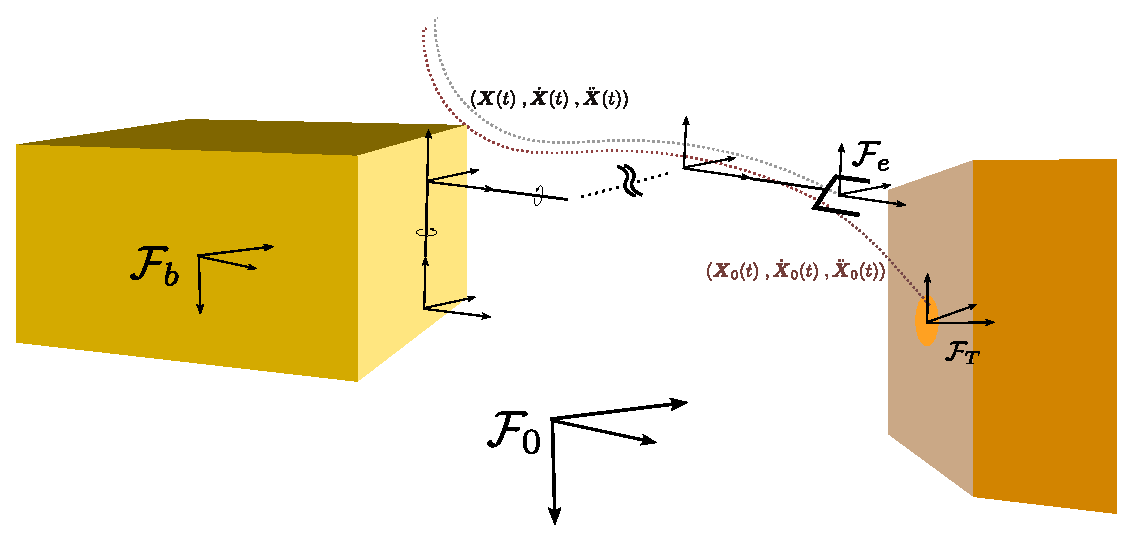
\includegraphics[scale=0.7]{./figures/uvms_kinematics_force.eps}
	\caption{Frames of the UVMS with the inertial and task frame}
	\label{fig:uvms_force}
\end{figure}
The force control is analyzed in the task space, as observed by the end effector, and we can define the forces acting upon the manipulator due to contact with the environment 
\begin{align}
	\bs F_e^e&=\begin{bmatrix} f_x & f_y & f_z & m_x & m_y & m_z \end{bmatrix}
	\label{eq:force_force}
\end{align}
$\bs F_e^e$ is therefor the same as $\bs F$ defined in \eqref{eq:jacobian_force} and can therefor be mapped into the joint the general forces $\taub$ by the transpose jacobian
\begin{align}
	\taub&=(\jb{ge}{B})^T\bs F_e^e
	\label{eq:jacobian-force2}
\end{align}
Let the translational part of the trajectory of the end effector be defined as

\begin{align}
	\bs X(t) \; , \; \dot{\bs X}(t)\; , \; \ddot{\bs X}(t)	
	\label{eq:ee_traj}
\end{align}
Which gives the position, velocity and acceleration of the end effector relative to the task frame \frame T, illustrated in Fig. \ref{fig:uvms_force}. Further we will define a nominal trajectory which represents the planned trajectory, given by a path plan algorithm and/or an operator

\begin{align}
	\bs X_0(t) \; , \; \dot{\bs X}_0(t)\; , \; \ddot{\bs X}_0(t)	
	\label{eq:nominal_force}
\end{align}
We can then model the force due to interaction, when the end effector is in contact with the environment, \cite{impedance_stability}

\begin{align}
	\bs F&=\bs K(\bs X - \bs X_0) + \bs B(\dot{\bs X} - \dot{\bs X}_0) + \bs J(\ddot{\bs X} - \ddot{\bs{X}}_0)
	\label{eq:ee_impedance1}
\end{align}
The nominal path can then be interpreted as the no contact path. The constants $\bs K$, $\bs B$ and $\bs J$ can then be regarded as the desired stiffness, damping and inertia of the end effector in contact with the environment. The impedance defined in \eqref{eq:nominal_force} can then be obtained either by direct force control, or it can be used to adjust the path of the endeffector, relying on an inner position control loop. In this paper the latter will be discussed. \cite{impedance_stability} proposes an adjustment vector $\bs X_a$ which is a result of filtering $\bs F$ through a second order low pass filter

\begin{align}
	\bs X_a(s)&= \frac{1}{(\bs K+\bs Bs+ \bs Js^2)}\bs F(s)
	\label{eq:x_adjusted}
\end{align}
$\bs X_a$ can then be seen as a perturbation from the nominal path due to the desired impedance, as defined in \eqref{eq:ee_impedance1}. We will, for the sake of simplicity only consider diagonal $\bs K$, $\bs B$ and $\bs J$ matrices, so that the forces are decoupled. The commanded trajectory that is used as the input for the motion control loop can then be written as
\begin{align}
	\bs X_c&= \bs X_0 + \bs X_a
	\label{eq:controlled_traj}
\end{align}





\section{Simulation}
\label{sec:simulation}
For testing the performance of the control strategies above, simulations where done using Matlab/Simulink running in an Linux environment. To provide a graphical representation of the UVMS, the \textit{Robotic Toolbox}\footnote{Robotic Toolbox is a toolbox for Matlab/Simulink written by Peter Corke, and distributed under the Lesser General Pulic Licence} where used. 
In the general setup of the simulation, an underwater vehicle was used, with a 6-link robotic manipulator mounted on. 
As recalled, only the inertia part of the dynamics is simulated (to to the assumption that the controller cancels out the nonlinear parts perfectly). The model of the uvms is therefor described by the matrix $\bs M(\bs q)$ and the DH-parameters.

\begin{table}[h!] % Add the following just after the closing bracket on this line to specify a position for the table on the page: [h], [t], [b] or [p] - these mean: here, top, bottom and on a separate page, respectively
\caption{DH parameters of the kinematic chain of the robot manipulator} % Table caption, can be commented out if no caption is required
\centering % Centers the table on the page, comment out to left-justify
\begin{tabular}{l c c c c } % The final bracket specifies the number of columns in the table along with left and right borders which are specified using vertical bars (|); each column can be left, right or center-justified using l, r or c. To specify a precise width, use p{width}, e.g. p{5cm}
\toprule % Top horizontal line
%& \multicolumn{3}{c}{DH parameters} \\ % Amalgamating several columns into one cell is done using the \multicolumn command as seen on this line
%\cmidrule(l){1-5} % Horizontal line spanning less than the full width of the table - you can add (r) or (l) just before the opening curly bracket to shorten the rule on the left or right side
Link & $ a_i $ & $ \alpha_i $ & $ d_i $ & $ \theta_i$ \\ % Column names row
\midrule % In-table horizontal line
1 & 0.2 & $\frac{\pi}{2}$ & 0 & $q_{1}$ \\ % Content row 1
2 & 1 &0 & 0 & $q_{2}$ \\ % Content row 2
3 & 0.6 & 0 & 0 & $q_{3}$ \\ % Content row 3
4 & 0.4 & $-\frac{\pi}{2}$ & 0 & $q_{4}$ \\ % Content row 4
5 & 0 & $-\frac{\pi}{2}$ & 0 & $q_{5}$ \\ % Content row 5
6 & 0 & 0& 0.4 & $q_{6}$ \\ % Content row 5
\bottomrule % Bottom horizontal line
\end{tabular}
\label{tab:template} % A label for referencing this table elsewhere, references are used in text as \ref{label}
\end{table}
Further, the origin of the vehicle frame \frame b is located at the base of the manipulator. Both a simulation of the force based path correction and the inverse kinematics is presented below. 

\subsection{Inverse Kinematics}

A simulation is done in order to test the inverse kinematic control law using the weighted pseudo inverse. The objective is to track an elliptic path that lies in the $x-z$ plane of the workspace of the end effector. 

\begin{figure}[h!]
	\centering
	\includegraphics[scale=0.5]{./figures/matlab/kinematic-sim1.eps}
	
	\caption{The objective of the simulation is to track the elliptic path (red) in the workspace of the end effector }
	\label{fig:robot-sim1}
\end{figure}


\begin{figure}[h!]
	\centering
	\includegraphics[scale=0.6]{./figures/matlab/kinematic-sim2.eps}
	
	\caption{Plot of commanded vehicle position and joint angles }
	\label{fig:robot-sim2}
\end{figure}

From Fig. \ref{fig:robot-sim2} one can see that the vehicle is close to stationary as long as the manipulator joints are away from their limits, and the path is within reach. Between $t=0 s$ and $t=1.2 s$ the vehicle has to move, in the x direction, in order for the end effector to reach the desired trajectory. After $t=1.2 s$ it is almost stationary. Then at $t=3 s $ $ q_{3}$ is getting close to its limit at $-110^{o}$ and the vehicle is commanded in the x-direction due to the loss of redundancy of the manipulator. The different configurations of the UVMS during the tracking can be seen in Fig. \ref{fig:robo-tracking}.  


\newcommand{\rscale}{0.18}
\begin{figure}[h!]
	\centering
%	\begin{subfigure}

		\includegraphics[scale=\rscale]{./figures/matlab/kin-robot101.eps}
%\end{subfigure}
%	\begin{subfigure}
		\includegraphics[scale=\rscale]{./figures/matlab/kin-robot161.eps}
		\includegraphics[scale=\rscale]{./figures/matlab/kin-robot261.eps} \\
	
		\includegraphics[scale=\rscale]{./figures/matlab/kin-robot361.eps}
		\includegraphics[scale=\rscale]{./figures/matlab/kin-robot461.eps}
		\includegraphics[scale=\rscale]{./figures/matlab/kin-robot561.eps} \\
		
		\includegraphics[scale=\rscale]{./figures/matlab/kin-robot661.eps}
		\includegraphics[scale=\rscale]{./figures/matlab/kin-robot761.eps}
		\includegraphics[scale=\rscale]{./figures/matlab/kin-robot861.eps}
		\\
		\includegraphics[scale=\rscale]{./figures/matlab/kin-robot961.eps}
		\includegraphics[scale=\rscale]{./figures/matlab/kin-robot1061.eps}
		\includegraphics[scale=\rscale]{./figures/matlab/kin-robot1161.eps}
		
%\end{subfigure}
	\caption{UVMS tracking the desired path}
	\label{fig:robo-tracking}
\end{figure}

\begin{figure}[h!]
	\centering
	\includegraphics[scale=0.6]{./figures/matlab/kinematic-sim3.eps}
	
	\caption{Plot of joint velocities and the elements of $W$ }
	\label{fig:robot-sim3}
\end{figure}

In the simulation above, the weighted pseudo inverse was used, where the matrix $W$ was weighted according to (citation needed). In Fig. \ref{fig:robot-sim3} one can see that both the joint velocities, and the diagonal elements of the weighting matrix $W$. When the joints are close to a limit, and the direction of the joint velocity changed, and thus switching the sign of $\Delta |\frac{\delta H}{\delta q_{i}}|$ it gives a very large change in the corresponding element of $W$. 
This will in turn cause oscillation in the joint velocities. This is due to the discretization of the system. In the continuous case the joint velocity is exactly 0 when $\Delta |\frac{\delta H}{\delta q_{i}}|$ changes sign. In the discrete case, however, the joint velocity is not necessary zero, and the large change in $W$ when the joint velocity is nonzero gives oscillations. 


\subsection{Force Based Motion Control}


\clearpage
\newpage
\bibliographystyle{plainnat}	% (uses file "plain.bst")
\bibliography{myrefs}		% expects file "myrefs.bib"

%\input{appendix.tex}
\end{document}
